% Tracking of Objects

\section{Tracking}
The system is using a background segmentation which have a certain learning rate, this means that the system constantly learns what is considered background during runtime. The background modelling will however not be able to handle all kinds of situations. There is, for example, a theoretical possibility for a person to walk into the scene, stand still for a sufficient period of time and blend into the background. This problem is solved by the use of a tracker which tracks objects found in the scene. The tracking algorithm will save information of objects that disappears in the scene and the robot will not continue working in normal pace until the object has left the safety zone. The system is not required to keep track of objects that is occluded and objects that interfere with each other. Since the requirement of the tracker is rather low the implementation is simple and has no guarantees of actually tracking objects throughout the entire scene if occlusion occurs.

To keep track of all objects in the scene an object list is used containing a vector of all objects and an index towards the object which is closest to the robot. Every object contains the closest joint on the robot, closest point on the object and the distance between them, which is called the min-distance. It will also contain an average point and a bool-variable which tells if the object is visible or not.  Every cluster which is classified as an object will then correspond to an object in the objectlist. When an object is calculated in a new frame its average point will be compared to the average points of the objects in the objectlist. If there are any objects in the objectlist which doesn’t correspond to any objects in the current frame there are theoretically two different possibilities, the object has moved out of the camera view or the object has blended into the background. To know which one it is the min-distance of the object is used. If the distance is sufficiently large it is assumed that the object has moved out of the camera view and the object will then be removed from the objectlist. If the distance is sufficiently small the object is assumed to have blended into the background, the object will then be kept in the objectlist but it will be marked as not visible. Objects that are outside the safety zones are not really interesting and will not be tracked. Since new objects can’t occur inside the safety zones another advantage with the tracking is that it will reduce noise.

\begin{figure}[H]
\begin{center}
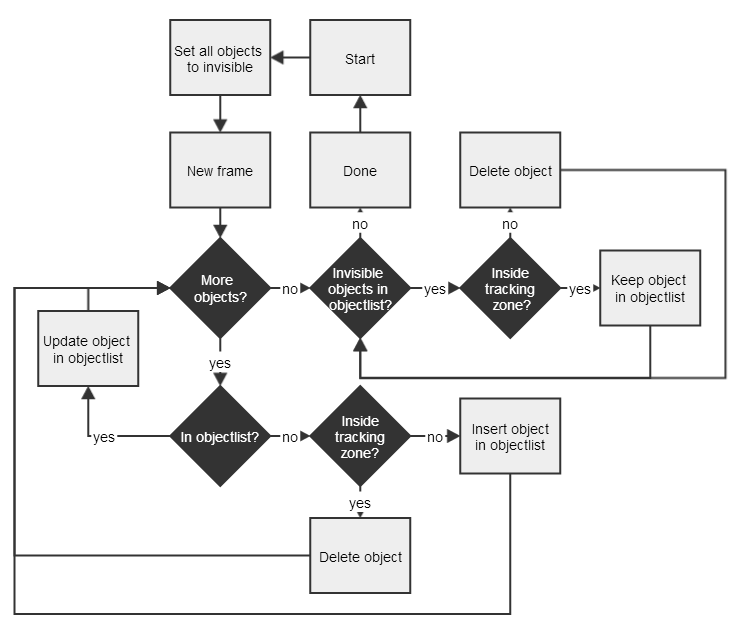
\includegraphics[width=12 cm]{tracking}
\caption{Flowchart of tracking algorithm}
\label{tracking}
\end{center}
\end{figure}
